\documentclass[12pt]{article}
\usepackage[paper=letterpaper,margin=1.5cm]{geometry}
\usepackage{amsmath}
\usepackage{amssymb}
\usepackage{amsfonts}
\usepackage{newtxtext, newtxmath}
\usepackage{enumitem}
\usepackage{titling}
\usepackage{svg}
\usepackage{xcolor}
\usepackage{listings}
\usepackage{float}
\usepackage{nicefrac}
\usepackage[most]{tcolorbox}
\usepackage[colorlinks=true]{hyperref}

\setlength{\droptitle}{-6em}

\definecolor{codegreen}{rgb}{0,0.6,0}
\definecolor{codegray}{rgb}{0.5,0.5,0.5}
\definecolor{codepurple}{rgb}{0.58,0,0.82}
\definecolor{backcolour}{rgb}{0.95,0.95,0.92}
\definecolor{bg}{rgb}{1,0.96,0.9}

\lstdefinestyle{mystyle}{
  commentstyle=\color{codegreen},
  keywordstyle=\color{magenta},
  numberstyle=\tiny\color{codegray},
  stringstyle=\color{codepurple},
  basicstyle=\ttfamily\footnotesize,
  breakatwhitespace=false,
  breaklines=true,
  captionpos=b,
  keepspaces=true,
  numbers=left,
  numbersep=5pt,
  showspaces=false,
  showstringspaces=false,
  showtabs=false,
  tabsize=2
}

% \tcbset{enlarge left by=-0.8cm,left=1.2cm,enlarge right by=-2cm,right=0.8cm}

\lstset{
  style=mystyle,
  inputencoding=utf8,
  extendedchars=true,
}

\begin{document}

The perceptron algorithm consists of one of the simplest types of neural
network architectures. It is a single-layer neural network with a single
neuron. The neuron is a linear combination of the input variables, with a
bias term, and then passed through an activation function. The activation
function is used to determine the output of the neuron.
The algorithm itself is a supervised learning algorithm, meaning that it
requires labeled training data to train the model. The algorithm is
iterative, hence it'll continue to update the weights until the
model converges. The learning rate is a hyperparameter that controls the
step size of the weight updates. The activation function is a hyperparameter
that determines the output of the neuron. The learning rule is as follows:

\begin{equation*}
  w^{new} \leftarrow w^{old} + \eta \cdot (z - \hat{z}(x)) \cdot x, \quad
  \hat{z}(x) = f(net(x)), \quad
  net(x) = \sum_{i=1}^n w_i \cdot x^{(i)} + w_0
\end{equation*}

where $w_i$ is the weight for the $i$th input variable, $\eta$ is the
learning rate, $z$ is the true label, $\hat{z}$ is the predicted label,
and $x_i$ is the $i$th input variable. The learning rule is applied for
each training example, and an epoch is a single pass through the entire
training set.

\begin{enumerate}[leftmargin=\labelsep]
  \begin{tcolorbox}[enhanced jigsaw,colback=bg,boxrule=0pt,arc=1pt,halign=center]
    \item Considering the following linearly separable training data:

    \begin{table}[H]
      \centering
      \begin{tabular}{c|c|c|c|c}
              & $y_1$ & $y_2$ & $y_3$ & $z$ \\ \hline
        $x_1$ & 0     & 0     & 0     & -1  \\
        $x_2$ & 0     & 2     & 1     & 1   \\
        $x_3$ & 1     & 1     & 1     & 1   \\
        $x_4$ & 1     & -1    & 0     & -1
      \end{tabular}
    \end{table}

    Given the perceptron learning algorithm with a learning rate $\eta = 1$,
    sign activation and all weights initialized to one (including the bias):

    \begin{enumerate}
      \item Considering $y_1$ and $y_2$, apply the algorithm until convergence.
            Draw the separation hyperplane.
      \item Considering all input variables, apply one epoch of the algorithm.
            Do weights change for an additional epoch?
      \item Identify the perceptron output for $x_{new}$ = $\begin{bmatrix} 0 & 0 & 1 \end{bmatrix}^T$.
      \item What happens if we replace the sign function with the step function? Specifically,
            how would you change $\eta$ to ensure the same results?
    \end{enumerate}
  \end{tcolorbox}

  \begin{enumerate}
    \item {
          As per the question statement, we're working with $\eta = 1$ and sign activation:

          $$
            \hat{z} = f(net) = \begin{cases}
              1  & net \geq 0 \\
              -1 & net < 0
            \end{cases}
          $$

          Moreover, we're considering weights (and the bias, $w_0$) initialized at one.
          Performing epochs following the $\{x_1, \cdots, x_4\}$ order, we get the following
          weight updates:

          \begin{align*}
            \hat{z}(x_1) & = f(net(x_1)) = f(1 + 1 \cdot 0 + 1 \cdot 0) = f(1) = 1                                                                                     \\
            x_1: \quad   & w \leftarrow \begin{bmatrix}
  0.1 & 0.1 & 0.1 & 0.1\\
  0.1 & 0.1 & 0.1 & 0.1\\
  0.1 & 0.1 & 0.1 & 0.1\\
  0.1 & 0.1 & 0.1 & 0.1\\
\end{bmatrix} + 1 \cdot (-1 - 1) \cdot \begin{bmatrix}
  1 & 0 & 0\\
\end{bmatrix}^T = \begin{bmatrix}
  -0.926984\\
  -2.90718\\
  -4.91178\\
\end{bmatrix} \\
            \hat{z}(x_2) & = f(net(x_2)) = f(-1 + 1 \cdot 0 + 1 \cdot 2) = f(1) = 1                                                                                    \\
            x_2: \quad   & w \leftarrow \begin{bmatrix}
  -0.926984\\
  -2.90718\\
  -4.91178\\
\end{bmatrix} + 1 \cdot (1 - 1) \cdot \begin{bmatrix}
  1 & 0 & 2\\
\end{bmatrix}^T = \begin{bmatrix}
  -1\\
  1\\
  1\\
\end{bmatrix}  \\
            \hat{z}(x_3) & = f(net(x_3)) = f(-1 + 1 \cdot 1 + 1 \cdot 1) = f(1) = 1                                                                                    \\
            x_3: \quad   & w \leftarrow \begin{bmatrix}
  -1\\
  1\\
  1\\
\end{bmatrix} + 1 \cdot (1 - 1) \cdot \begin{bmatrix}
  1 & 1 & 1\\
\end{bmatrix}^T = \begin{bmatrix}
  -1\\
  1\\
  1\\
\end{bmatrix}  \\
            \hat{z}(x_4) & = f(net(x_4)) = f(-1 + 1 \cdot 1 + 1 \cdot -1) = f(-1) = -1                                                                                 \\
            x_4: \quad   & w \leftarrow \begin{bmatrix}
  -1\\
  1\\
  1\\
\end{bmatrix} + 1 \cdot (-1 + 1) \cdot \begin{bmatrix}
  1 & 1 & -1\\
\end{bmatrix}^T = \begin{bmatrix}
  -1\\
  1\\
  1\\
\end{bmatrix}
          \end{align*}

          After entering a new epoch, we'd update the weights again, this time for $x_1$;
          since such an update wouldn't lead to an actual update on the weight matrix,
          that'd make a full pass on the training set without changes, and, as such,
          the algorithm would converge. Therefore, the regression hyperplane is given by:

          $$
            -1 + x_1 + x_2 = 0 \leftrightarrow x_2 = 1 - x_1
          $$

          % TODO: Plotting the data and the hyperplane, we get the following:
          }
    \item {
          Here, we apply the same algorithm as before, but now considering all input variables.

          \begin{align*}
            \hat{z}(x_1) & = f(net(x_1)) = f(1 + 1 \cdot 0 + 1 \cdot 0 + 1 \cdot 0) = f(1) = 1                                                                         \\
            x_1: \quad   & w \leftarrow \begin{bmatrix}
  1\\
  1\\
  1\\
  1\\
\end{bmatrix} + 1 \cdot (-1 - 1) \cdot \begin{bmatrix}
  1 & 0 & 0 & 0\\
\end{bmatrix}^T = \begin{bmatrix}
  -1\\
  1\\
  1\\
  1\\
\end{bmatrix} \\
            \hat{z}(x_2) & = f(net(x_2)) = f(-1 + 1 \cdot 0 + 1 \cdot 2 + 1 \cdot 1) = f(2) = 1                                                                        \\
            x_2: \quad   & w \leftarrow \begin{bmatrix}
  -1\\
  1\\
  1\\
  1\\
\end{bmatrix} + 1 \cdot (1 - 1) \cdot \begin{bmatrix}
  0\\
  1\\
\end{bmatrix}^T = \begin{bmatrix}
  -1\\
  1\\
  1\\
  1\\
\end{bmatrix}  \\
            \hat{z}(x_3) & = f(net(x_3)) = f(-1 + 1 \cdot 1 + 1 \cdot 1 + 1 \cdot 1) = f(2) = 1                                                                        \\
            x_3: \quad   & w \leftarrow \begin{bmatrix}
  -1\\
  1\\
  1\\
  1\\
\end{bmatrix} + 1 \cdot (1 - 1) \cdot \begin{bmatrix}
  1 & 1 & 1 & 1\\
\end{bmatrix}^T = \begin{bmatrix}
  -1\\
  1\\
  1\\
  1\\
\end{bmatrix}  \\
            \hat{z}(x_4) & = f(net(x_4)) = f(-1 + 1 \cdot 1 + 1 \cdot -1 + 1 \cdot 0) = f(-1) = -1                                                                     \\
            x_4: \quad   & w \leftarrow \begin{bmatrix}
  -1\\
  1\\
  1\\
  1\\
\end{bmatrix} + 1 \cdot (-1 + 1) \cdot \begin{bmatrix}
  2\\
  2\\
\end{bmatrix}^T = \begin{bmatrix}
  -1\\
  1\\
  1\\
  1\\
\end{bmatrix}
          \end{align*}

          Once again, we'd enter a new epoch and update the weights considering the first sample,
          but since such an update wouldn't lead to an actual update on the weight matrix,
          that'd make a full pass on the training set without changes, and, as such,
          the algorithm would converge. \textbf{An additional epoch wouldn't, therefore,
            change the weights}.
          }
    \item {
          As we've mentioned before, the perceptron's output is given by the
          activation function - here, the sign of the net input. Therefore, the
          perceptron's output is given by:

          $$
            \hat{z} = f(net) = \begin{cases}
              1  & net \geq 0 \\
              -1 & net < 0
            \end{cases}
          $$

          Here, considering the weights computed in the previous question, we'll
          have the following:

          $$
            net(x_{new}) = -1 + 1 \cdot 0 + 1 \cdot 0 + 1 \cdot 1 = 0
          $$

          As we know, $f(0) = 1$, and, as such, the perceptron would classify the
          new sample as belonging to the binary class $1$.
          }
    \item {
          As we know, the step function is rather similar to the sign function,
          defined as follows:

          $$
            f(net) = \begin{cases}
              1 & net \geq 0 \\
              0 & net < 0
            \end{cases}
          $$

          Let's consider the following learning rules (the first one considers
          the activation function as the sign function, and the second one
          considers the activation function as the step function):

          \begin{align*}
            \text{Sign function:} \quad & w \leftarrow w + \eta \cdot (z - sign(net)) \cdot x \\
            \text{Step function:} \quad & w \leftarrow w + \eta \cdot (z - step(net)) \cdot x
          \end{align*}

          We can note, of course, that the only differing term between both rules
          is $(z - \hat{z})$; therefore, to make it so that both rules are
          equivalent, we'd have to make sure that the step function's output
          is correctly balanced with the sign function's output, utilizing a scalar
          factor (be it $\tau$) for such purpose, effectively altering the learning
          rate to be $\eta_{sign} = \tau \cdot \eta_{step}$. Let's try to find $\tau$:

          $$
            z - sign(net) = \tau (z - step(net))
          $$

          Note that, when using the step function, we should map the target from
          $z \in \{-1, 1\}$ to $z \in \{0, 1\}$ (since it wouldn't make sense to
          estimate other kinds of values), and, as such, we can write
          the following:

          \begin{align*}
            z - sign(net) & = \begin{cases}
                                1 - 1 = 0  & net \geq 0 \text { and } z = 1  \\
                                -1 -1 = -2 & net \geq 0 \text { and } z = -1 \\
                                1 + 1 = 2  & net < 0 \text { and } z = 1     \\
                                -1 + 1 = 0 & net < 0 \text { and } z = -1
                              \end{cases}, \quad
            z - step(net) & = \begin{cases}
                                1 - 1 = 0  & net \geq 0 \text { and } z = 1 \\
                                0 - 1 = -1 & net \geq 0 \text { and } z = 0 \\
                                1 - 0 = 1  & net < 0 \text { and } z = 1    \\
                                0 - 0 = 0  & net < 0 \text { and } z = 0
                              \end{cases}
          \end{align*}

          As such, if we want an equal learning rule utilizing both step and sign
          functions, we'd have to set $\tau = 2$, as can be trivially deduced from
          the cases above. With all this said, we'll get the following learning rule:

          $$
            w \leftarrow w + 2 \eta_{sign} \cdot (z - step(net)) \cdot x \quad \leftrightarrow \quad
            w \leftarrow w + \eta_{sign} \cdot (z - sign(net)) \cdot x
          $$
          }
  \end{enumerate}

  \begin{tcolorbox}[enhanced jigsaw,colback=bg,boxrule=0pt,arc=1pt,halign=center]
    \item Let us consider the following activation function and training set:

    \begin{equation*}
      \hat{z}(x, w) = \frac{1}{1 + e^{-2 w x}}
    \end{equation*}

    \begin{table}[H]
      \centering
      \begin{tabular}{c|c|c|c}
              & $y_1$ & $y_2$ $z$       \\ \hline
        $x_1$ & $1$   & $1$       & $1$ \\
        $x_2$ & $2$   & $1$       & $1$ \\
        $x_3$ & $1$   & $3$       & $0$ \\
        $x_4$ & $3$   & $3$       & $0$
      \end{tabular}
    \end{table}

    Consider also the half sum of squared errors as the loss function:

    \begin{equation*}
      E(w) = \nicefrac{1}{2} \sum_{i=1}^N (z_i - \hat{z}(x_i, w))^2
    \end{equation*}

    \begin{enumerate}
      \item Determine the gradient descent learning rule for this unit.
      \item Compute the first gradient descent update, assuming an initialization of all ones.
      \item Compute the first stochastic gradient descent update assuming an initialization of all ones.
    \end{enumerate}
  \end{tcolorbox}

  As we should know by now, (activation) functions of the type $\frac{1}{1 + e^{-k}}$
  are called sigmoid functions - functions that are bounded by $0$ and $1$,
  with $\sigma(0) = 0.5$. $\sigma(x)$ is plotted below:

  \begin{figure}[h]
    \centering
    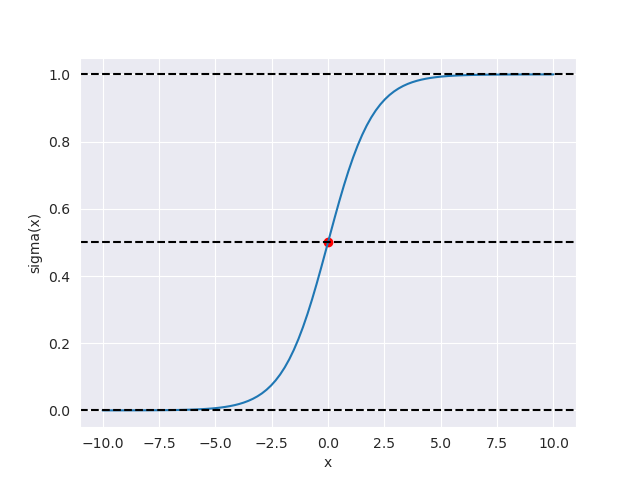
\includegraphics[width=0.5\textwidth]{assets/sigmoid.png}
    \caption{Sigmoid function}
  \end{figure}

  Sigmoid functions are widely used in Machine Learning (and, in particular, in
  perceptrons/neural network nodes) since they're able to map any real number
  to the interval $[0, 1]$, and, as such, they're able to represent probabilities
  fairly well. The sigmoid's derivative is rather famous (and must be known
  for the exam), given by:

  $$
    \frac{\partial \sigma(\alpha x)}{\partial w} = \alpha \sigma(\alpha x) (1 - \sigma(\alpha x)
  $$

  Gradient descent is essentially a linear regression
  model where, once again, we try to minimize a given error function - if in the case
  of the previous perceptron learning rule this error function was simply the
  difference between the desired output and the perceptron's output, in the case
  of gradient descent we have a more complex error function, such as the half
  sum of squared errors. We utilize this more complex learning rule when, for example,
  we're in the presence of non-linearly separable data, and, as such, we can't
  use the perceptron learning rule to find a separating hyperplane. Here, the
  learning rule is written as follows (considering $E$ as the error function):

  $$
    w \leftarrow w - \eta \cdot \frac{\partial E}{\partial w}
  $$

  Note that here, since we're working with gradient \textbf{descent}, we're now
  subtracting the gradient of the error function from the weights, instead of
  adding it - we're trying to minimize the error function, after all.

  \begin{enumerate}
    \item {
          Note that the activation function, here, is a sigmoid that not only depends
          on $x$ but also $w$:

          $$
            \hat{z}(x, w) = \sigma(2wx) =  \frac{1}{1 + e^{-2 w x}}
          $$

          Let's try to derivate the error function with respect to $w$:

          \begin{align*}
            \frac{\partial E}{\partial w} & = \frac{\partial}{\partial w} \frac{1}{2} \sum_{i=1}^N (z_i - \hat{z}(x_i, w))^2                       \\
                                          & = \frac{2}{2} \sum_{i=1}^N (z_i - \hat{z}(x_i, w)) \frac{\partial}{\partial w} (z_i - \hat{z}(x_i, w)) \\
                                          & = - \sum_{i=1}^N (z_i - \sigma(2wx_i)) \sigma(2wx_i) (1 - \sigma(2wx_i)) 2x_i                          \\
                                          & = -2 \sum_{i=1}^N x_i (z_i - \sigma(2wx_i)) \sigma(2wx_i) (1 - \sigma(2wx_i))
          \end{align*}

          Therefore, our learning rule will be written as:

          $$
            w \leftarrow w + 2\eta \sum_{i=1}^N x_i (z_i - \sigma(2wx_i)) \sigma(2wx_i) (1 - \sigma(2wx_i)))
          $$
          }
    \item {

          \textit{\textbf{Note:} On all matrix dot products between $x_i$'s and $w$, in this and
            the following questions, we're considering here for it to be the dot product between
            $x_i$ and the \textbf{transposed} of $w$, since otherwise the dimensions wouldn't match
            (probably an issue regarding the original question's statement).}

          Considering an initialization of all ones, we have the following:

          $$
            \eta = 1, \quad w = \begin{bmatrix}
  0\\
  1\\
  0\\
\end{bmatrix}, \quad X = \begin{bmatrix}
  1 & 3 & -1\\
  1 & 4 & 2\\
  1 & 2 & 2\\
\end{bmatrix}
          $$

          Here, we're asked to compute the first gradient descent update - i.e,
          the first update of the weights after the first epoch. As such, we'll have
          the following (computations in this sheet's notebook):

          \begin{align*}
            w & \leftarrow w + 2 \eta \sum_{i=1}^N x_i (z_i - \sigma(2wx_i)) \sigma(2wx_i) (1 - \sigma(2wx_i))) \\
              & \leftarrow \begin{bmatrix}
  0\\
  1\\
  0\\
\end{bmatrix} + 2 \cdot 1 \cdot
            \left(
            \begin{bmatrix}
  1 & 0 & 0 & 0\\
\end{bmatrix} \cdot \left(
              1 - \sigma(2 \cdot \begin{bmatrix}
  0\\
  1\\
  0\\
\end{bmatrix} \cdot \begin{bmatrix}
  1 & 0 & 0 & 0\\
\end{bmatrix})
              \right) \cdot \sigma(2 \cdot \begin{bmatrix}
  0\\
  1\\
  0\\
\end{bmatrix} \cdot \begin{bmatrix}
  1 & 0 & 0 & 0\\
\end{bmatrix}) \cdot
            \left(1 - \sigma(2 \cdot \begin{bmatrix}
  0\\
  1\\
  0\\
\end{bmatrix} \cdot \begin{bmatrix}
  1 & 0 & 0 & 0\\
\end{bmatrix})\right)
            + \cdots \right) = \begin{bmatrix}
  -0.926984\\
  -2.90718\\
  -4.91178\\
\end{bmatrix}
          \end{align*}

          }
    \item {
          If in the previous question, with a batch gradient descent update, we
          computed the weight update for the whole first epoch at once, with
          stochastic gradient descent we'll compute the weight update for each
          sample individually - the "sum" in the learning rule, here, will be replaced
          by a single sample, as can be seen below:

          $$
            w \leftarrow w + 2\eta x_1 (z_1 - \sigma(2wx_1)) \sigma(2wx_1) (1 - \sigma(2wx_1))
          $$

          This will be essentially calculating the expression written in the question above
          (before the $\cdots$), which ends up updating the weight matrix to the following:

          $$
            w_{new} = \begin{bmatrix}
  1.04743\\
  1.04743\\
  1.04743\\
\end{bmatrix}
          $$
          }
  \end{enumerate}

  \begin{tcolorbox}[enhanced jigsaw,colback=bg,boxrule=0pt,arc=1pt,halign=center]
    \item Let us consider the following activation function, with the training data set
    from the previous exercise:

    \begin{equation*}
      \hat{z}(x, w) = \frac{1}{1 + e^{-w x}}
    \end{equation*}

    Here, we'll be using the cross-entropy loss function:

    \begin{equation*}
      E(w) = - \sum_{i=1}^N z_i \log \hat{z}(x_i, w) + (1 - z_i) \log (1 - \hat{z}(x_i, w))
    \end{equation*}

    \begin{enumerate}
      \item Determine the gradient descent learning rule for this unit.
      \item Compute the first gradient descent update, assuming an initialization of all ones.
      \item Compute the first stochastic gradient descent update assuming an initialization of all ones.
    \end{enumerate}
  \end{tcolorbox}

  \begin{enumerate}
    \item {
          Here, we'll compute the learning rule for the gradient descent the same way,
          with the exception of the gradient of the error function, of course: here,
          we're working with the cross-entropy loss function, instead of the squared
          error function. After a fantastic derivation, we'll have the following:

          $$
            E(w) = - \log(P(z|x, w)) = - \sum_{i=1}^N (z_i \log \hat{z}(x_i, w) + (1 - z_i) \log (1 - \hat{z}(x_i, w)))
          $$
          $$
            \frac{\partial E}{\partial w} = - \sum_{i=1}^N \left(
            \frac{z_i (\hat{z}(x_i, w))'}{\hat{z}(x_i, w)} + \frac{(z_i - 1) (\hat{z}(x_i, w))'}{1 - \hat{z}(x_i, w)}
            \right)
          $$

          In our case, considering that the activation function is a sigmoid once again
          (this time $\sigma(wx)$), we'll have:

          $$
            \frac{\partial \hat{z}}{\partial w} = x_i \sigma(w x_i) (1 - \sigma(w x_i))
          $$

          Therefore, the gradient for the loss function will be given by:

          \begin{align*}
            \frac{\partial E}{\partial w} & = - \sum_{i=1}^N \left(
            \frac{z_i x_i \sigma(w x_i) (1 - \sigma(w x_i))}{\sigma(w x_i)} +
            \frac{(z_i - 1) x_i \sigma (w x_i) (1 - \sigma(w x_i))}{1 - \sigma(w x_i)}
            \right)                                                                                                    \\
                                          & = - \sum_{i=1}^N z_i x_i (1 - \sigma(w x_i)) + (z_i - 1) x_i \sigma(w x_i) \\
                                          & = - \sum_{i=1}^N x_i \left(
            z_i - z_i \sigma(w x_i) + z_i \sigma(w x_i) - \sigma(w x_i)
            \right) = - \sum_{i=1}^N x_i (z_i - \sigma(w x_i))
          \end{align*}

          As such, the learning rule will be:

          $$
            w \leftarrow w + \eta \sum_{i=1}^N x_i (z_i - \sigma(w x_i))
          $$
          }
    \item {
          Once again, regarding an initialization of all ones, we'll have the following:

          $$
            \eta = 1, \quad w = \begin{bmatrix}
  0\\
  1\\
  0\\
\end{bmatrix}
          $$

          Now, with the new learning rule, we'll be able to write the first batch
          gradient descent update as:

          $$
            w \leftarrow w + \eta \sum_{i=1}^N x_i (z_i - \sigma(w x_i))
            = \begin{bmatrix}
  0\\
  1\\
  0\\
\end{bmatrix} + 1 \cdot \left(
            \begin{bmatrix}
  1 & 0 & 0 & 0\\
\end{bmatrix} \cdot \left(
              1 - \sigma(\begin{bmatrix}
  0\\
  1\\
  0\\
\end{bmatrix} \cdot \begin{bmatrix}
  1 & 0 & 0 & 0\\
\end{bmatrix})
              \right)
            + \cdots \right) = \begin{bmatrix}
  -0.926984\\
  -2.90718\\
  -4.91178\\
\end{bmatrix}
          $$

          }
    \item {
          Once again, with a stochastic gradient descent update, we'll compute the weight update
          for each sample individually - here, considering the \textbf{first} update,
          we're only going to consider the first sample. As such, we'll have:

          $$
            w \leftarrow w + \eta x_1 (z_1 - \sigma(w x_1)) = \begin{bmatrix}
  1.04743\\
  1.04743\\
  1.04743\\
\end{bmatrix}
          $$
          }
  \end{enumerate}

  \begin{tcolorbox}[enhanced jigsaw,colback=bg,boxrule=0pt,arc=1pt,halign=center]
    \item Consider now the half sum of squared errors loss function, paired with
    the following activation function:

    $$
      \hat{z}(x, w) = e^{(w x)^2}
    $$

    \begin{enumerate}
      \item Determine the gradient descent learning rule for this unit.
      \item Compute the stochastic gradient descent update for input $x_{new}$ = $\begin{bmatrix} 1 & 1 \end{bmatrix}^T$,
            $z_{new} = 0$, with initial weights $w = \begin{bmatrix} 0 & 1 & 0 \end{bmatrix}^T$
            and learning rate $\eta = 2$.
    \end{enumerate}
  \end{tcolorbox}

  \begin{enumerate}
    \item {
          Once again, we'll have to compute the derivative of the loss function with
          respect to the weights. As such, we'll have:

          $$
            E(w) = \frac{1}{2} \sum_{i=1}^N (z_i - \hat{z}(x_i, w))^2
          $$
          $$
            \frac{\partial E}{\partial w} = \frac{\partial}{\partial w} \frac{1}{2} \sum_{i=1}^N (z_i - \hat{z}(x_i, w))^2 \\
            = \sum_{i=1}^N (z_i - \hat{z}(x_i, w)) \frac{\partial}{\partial w} (z_i - \hat{z}(x_i, w))
            = -2 \sum_{i=1}^N x_i (w x_i) (z_i - e^{(w x_i)^2}) e^{(w x_i)^2}
          $$

          Our learning will be, then:

          $$
            w \leftarrow w + 2\eta \sum_{i=1}^N x_i (w x_i) (z_i - e^{(w x_i)^2}) e^{(w x_i)^2}
          $$
          }
    \item {
          We're asked to perform a stochastic gradient descent update for a new query
          vector $x_{new} = \begin{bmatrix}1 & 1\end{bmatrix}^T$, with label $0$.
          Moreover, the weights are initialized as $w = \begin{bmatrix}0 & 1 & 0\end{bmatrix}^T$
          and the learning rate is $\eta = 2$. As such, and plugging these values
          onto our learning rule, we'll have the following:

          \begin{align*}
            w & \leftarrow w + 2\eta x_{new} (w x_{new}) (z_{new} - e^{(w x_{new})^2}) e^{(w x_{new})^2} \\
              & \leftarrow \begin{bmatrix}
  0\\
  1\\
  0\\
\end{bmatrix} + 2 \cdot 2 \cdot
            \begin{bmatrix}
  1 & 3 & -1\\
  1 & 4 & 2\\
  1 & 2 & 2\\
\end{bmatrix} \cdot \left(
            \begin{bmatrix}
  0\\
  1\\
  0\\
\end{bmatrix} \cdot \begin{bmatrix}
  1 & 3 & -1\\
  1 & 4 & 2\\
  1 & 2 & 2\\
\end{bmatrix}
            \right) \cdots                                                                               \\
              & \leftarrow \begin{bmatrix}
  1.04743\\
  1.04743\\
  1.04743\\
\end{bmatrix}
          \end{align*}

          }
  \end{enumerate}

  \begin{tcolorbox}[enhanced jigsaw,colback=bg,boxrule=0pt,arc=1pt,halign=center]
    \item Consider the sum squared and cross-entropy loss functions. Any stands out?
    What changes when one changes the loss function?
  \end{tcolorbox}

  \textit{Note: this answer was mostly written by \href{https://github.com/Calhau18}{João Rocha}.}

  The cross-entropy loss function stands out as it corresponds to making a MLE of
  the parameter $w$ under the assumption that the data is generated by a
  \href{https://resumos.leic.pt/pe/va-discretas#distribuição-de-bernoulli}{Bernoulli}
  distribution, such that the outputs $z$ are sampled from a random variable $Z$
  with probability $p(Z = 1) = \sigma(w x)$ and $p(Z = 0) = 1 - \sigma(w x)$.
  As such, the cross-entropy loss function is the negative log-likelihood
  of the data under such distribution.

  The sum of squares loss function would be more fitted to a regression scenario,
  since it matches a MLE estimation of $w$ under the assumption that the outputs
  $z$ are sampled from a random variable $Z \sim \mathcal{N} (wx, \sigma^2)$.
  Nevertheless, one can use the sum of squares loss function on classification problems as well - as
  a matter of fact, this function is also convex, thus the use of gradient descent
  will also find a global minimum. In this case, the difference between the functions
  will be the value of the minimal parameter: since the functions are different,
  most likely their minimal values will be different as well, leading to different
  estimations of the parameter $w$; regarding classification problems, like the one
  in hands, the cross-entropy loss function should generally lead to a better estimation
  of the parameter $w$.

\end{enumerate}

\end{document}